\documentclass[12pt, a4paper]{article}

% ── Packages ──────────────────────────────────────────────────────────────────
\usepackage[margin=2.5cm, top=3cm, bottom=3cm]{geometry}
\usepackage[table]{xcolor}
\usepackage{amsmath}
\usepackage{booktabs}
\usepackage{array}
\usepackage{tabularx}
\usepackage{graphicx}
\usepackage{hyperref}
\usepackage{fancyhdr}
\usepackage{titlesec}
\usepackage{parskip}
\usepackage{enumitem}
\usepackage[letterspace=150]{microtype}
\usepackage{mdframed}
\usepackage{lmodern}
\usepackage{fontenc}
\usepackage{inputenc}
\usepackage{caption}
\usepackage{subcaption}
\usepackage{float}
\usepackage{multirow}
\usepackage{longtable}
\usepackage{tcolorbox}
\tcbuselibrary{skins, breakable}

% ── Colours ───────────────────────────────────────────────────────────────────
\definecolor{ehaBlue}{RGB}{0, 84, 142}
\definecolor{ehaLightBlue}{RGB}{224, 237, 248}
\definecolor{ehaGrey}{RGB}{245, 245, 245}
\definecolor{ehaAccent}{RGB}{0, 153, 118}
\definecolor{ehaRed}{RGB}{192, 57, 43}
\definecolor{ehaAmber}{RGB}{230, 126, 34}
\definecolor{tableHead}{RGB}{0, 84, 142}
\definecolor{tableAlt}{RGB}{240, 248, 255}
\definecolor{mapeGreen}{RGB}{212, 237, 218}
\definecolor{mapeAmber}{RGB}{255, 243, 205}
\definecolor{mapeRed}{RGB}{248, 215, 218}

% ── Hyperlinks ────────────────────────────────────────────────────────────────
\hypersetup{
  colorlinks=true, linkcolor=ehaBlue, urlcolor=ehaBlue,
  pdftitle={Tier 1 \& 2 Demand Forecasting Report --- EHA Clinics},
  pdfauthor={Supply Chain Analytics},
}

% ── Header / Footer ───────────────────────────────────────────────────────────
\pagestyle{fancy}
\fancyhf{}
\fancyhead[L]{\small\textcolor{ehaBlue}{\textbf{EHA Clinics} $\mid$ Tier 1 \& 2 Demand Forecasting Report}}
\fancyhead[R]{\small\textcolor{gray}{May 2026}}
\fancyfoot[C]{\small\textcolor{gray}{\thepage}}
\renewcommand{\headrulewidth}{0.4pt}
\renewcommand{\headrule}{\hbox to\headwidth{\color{ehaBlue}\leaders\hrule height\headrulewidth\hfill}}
\setlength{\headheight}{25.4pt}

% ── Section styling ───────────────────────────────────────────────────────────
\titleformat{\section}{\large\bfseries\color{ehaBlue}}{\thesection.}{0.6em}{}[\titlerule]
\titleformat{\subsection}{\normalsize\bfseries\color{ehaBlue!80!black}}{\thesubsection}{0.6em}{}
\titleformat{\subsubsection}{\small\bfseries\color{ehaBlue!60!black}}{\thesubsubsection}{0.6em}{}
\titlespacing*{\section}{0pt}{1.6em}{0.7em}
\titlespacing*{\subsection}{0pt}{1.1em}{0.4em}
\titlespacing*{\subsubsection}{0pt}{0.9em}{0.3em}

% ── Callout boxes ─────────────────────────────────────────────────────────────
\mdfdefinestyle{keybox}{
  backgroundcolor=ehaLightBlue, linecolor=ehaBlue, linewidth=1pt,
  innerleftmargin=12pt, innerrightmargin=12pt,
  innertopmargin=10pt, innerbottommargin=10pt, roundcorner=4pt,
}
\mdfdefinestyle{warnbox}{
  backgroundcolor=ehaAmber!12, linecolor=ehaAmber, linewidth=1.5pt,
  topline=false, rightline=false, bottomline=false,
  innerleftmargin=12pt, innerrightmargin=12pt,
  innertopmargin=8pt, innerbottommargin=8pt,
}
\mdfdefinestyle{alertbox}{
  backgroundcolor=ehaRed!8, linecolor=ehaRed, linewidth=1.5pt,
  topline=false, rightline=false, bottomline=false,
  innerleftmargin=12pt, innerrightmargin=12pt,
  innertopmargin=8pt, innerbottommargin=8pt,
}
\mdfdefinestyle{greenbox}{
  backgroundcolor=ehaAccent!10, linecolor=ehaAccent, linewidth=1.5pt,
  topline=false, rightline=false, bottomline=false,
  innerleftmargin=12pt, innerrightmargin=12pt,
  innertopmargin=8pt, innerbottommargin=8pt,
}

% ── Table helpers ─────────────────────────────────────────────────────────────
\newcolumntype{L}[1]{>{\raggedright\arraybackslash}p{#1}}
\newcolumntype{C}[1]{>{\centering\arraybackslash}p{#1}}
\newcolumntype{R}[1]{>{\raggedleft\arraybackslash}p{#1}}

% ── Figure caption style ──────────────────────────────────────────────────────
\captionsetup{font=small, labelfont={bf,color=ehaBlue}, labelsep=period,
              skip=6pt, width=0.95\textwidth}

% ── Finding counter ───────────────────────────────────────────────────────────
\newcounter{finding}
\newcommand{\finding}[1]{%
  \stepcounter{finding}%
  \begin{mdframed}[style=greenbox]
  \textbf{Finding \thefinding:} #1
  \end{mdframed}%
}

\begin{document}

% ════════════════════════════════════════════════════════════════════════════════
%  TITLE PAGE
% ════════════════════════════════════════════════════════════════════════════════
\begin{titlepage}
  \pagecolor{ehaBlue}\color{white}
  \vspace*{1.8cm}

  {\fontsize{10}{12}\selectfont\MakeUppercase{\textls[100]{Analytical Report}}}\\[0.5em]
  {\fontsize{26}{32}\selectfont\bfseries Tier 1 \& Tier 2 Demand\\[0.3em]
   Forecasting Models}\\[1.2em]
  \textcolor{ehaAccent}{\rule{6cm}{2pt}}\\[1.2em]

  {\large Procurement Demand Forecasting Initiative}\\[0.4em]
  {\normalsize EHA Clinics $\cdot$ Supply Chain Analytics}\\[2.5cm]

  \begin{tabular}{@{}ll}
    \textbf{Document Version}  & 1.0 \\[0.4em]
    \textbf{Date}              & May 1, 2026 \\[0.4em]
    \textbf{Data source}       & Odoo ERP (exported CSV) \\[0.4em]
    \textbf{Training window}   & January 2021 -- December 2023 \\[0.4em]
    \textbf{Validation window} & January 2024 -- June 2024 \\[0.4em]
    \textbf{Status}            & Final --- Q2 Baseline \\
  \end{tabular}

  \vfill
  {\small\textcolor{white!70!ehaBlue}
    {This report documents the implementation and evaluation of Tier 1
     (Seasonal Na\"{i}ve, 12-Month Rolling Average) and Tier 2 (ETS,
     SARIMA, Theta) forecasting models across all eligible
     category-facility pairs. It establishes the official Q2 MAPE
     baseline and identifies which pairs require escalation to Tier 3
     (Prophet) to meet the KPI target of MAPE $\leq 20\%$.}}
\end{titlepage}
\pagecolor{white}\color{black}

% ════════════════════════════════════════════════════════════════════════════════
%  EXECUTIVE SUMMARY
% ════════════════════════════════════════════════════════════════════════════════
\newpage

\begin{mdframed}[style=keybox]
\textbf{\large Executive Summary}\\[0.6em]
This report presents the results of applying five forecasting models ---
two Tier 1 benchmarks and three Tier 2 classical models --- to all
\textbf{15 eligible category-facility pairs} at EHA Clinics' six pilot
facilities. Models were trained on the January 2021--December 2023
window and evaluated against actuals from January--June 2024.\\[0.5em]

Six key conclusions emerge from this evaluation:

\begin{enumerate}[leftmargin=1.5em, itemsep=3pt]
  \item \textbf{No pair meets the MAPE $\leq 20\%$ KPI at Tier 1 or Tier 2.}
        The best individual validation MAPE achieved is \textbf{44.8\%}
        (Vaccines at Kano Lamido, ETS). All 15 pairs require escalation
        to Tier 3 (Facebook Prophet).

  \item \textbf{ETS is the most broadly reliable Tier 2 model.}
        ETS (Holt-Winters) achieves the lowest validation MAPE for
        8 of 15 pairs, outperforming both SARIMA and Theta across the
        majority of categories. Theta is competitive for sparse series.

  \item \textbf{SARIMA is frequently pathological on short or sparse series.}
        Several pairs produce SARIMA MAPEs exceeding 1,000\%
        (Injections at Asba: 1,270\%; Consumables at Lamido: 1,539\%;
        Lab Consumables at Lamido: 17,519\%). This reflects numerical
        instability and over-differencing on low-volume series, not a
        poor underlying demand signal.

  \item \textbf{Vaccines at Kano Lamido is the best-performing pair} and
        the closest to the target. ETS achieves 44.8\% MAPE and SARIMA
        49.3\%. With Prophet's holiday and programme regressors, this
        pair is a strong candidate to meet MAPE $\leq 20\%$ at Tier 3.

  \item \textbf{Laboratory Consumables at Asba returned all-NaN MAPEs.}
        The validation series (Jan--Jun 2024) contains no non-zero
        procurement months for this pair, indicating a complete procurement
        halt. This is likely a data or operational anomaly, not a genuine
        zero-demand period, and requires investigation before modelling.

  \item \textbf{All 15 eligible pairs are escalated to Tier 3 (Prophet).}
        The Q2 baseline is now established: MAPE ranges from 44.8\% to
        $>$7,000\% depending on the pair and model. Q3 improvement
        targets should be set on a per-pair basis, not as a uniform
        target across all categories.
\end{enumerate}
\end{mdframed}

\newpage
\tableofcontents
\newpage

% ════════════════════════════════════════════════════════════════════════════════
%  1. INTRODUCTION
% ════════════════════════════════════════════════════════════════════════════════
\section{Introduction}

\subsection{Purpose and Context}

This report presents the quantitative results of the Tier 1 and Tier 2
modelling phase of the EHA Clinics Procurement Demand Forecasting
Initiative. It builds directly on two predecessor documents:

\begin{itemize}[leftmargin=1.5em, itemsep=3pt]
  \item \textbf{Forecasting Scope and Modelling Approach} (Concept Note,
        April 2026) --- which defined the commodity and facility scope,
        training and validation windows, the tiered modelling strategy,
        and the KPI target of MAPE $\leq 20\%$ per category-facility pair.

  \item \textbf{Exploratory Data Analysis Report} (April 2026) --- which
        characterised demand patterns, identified the Kano Independence
        Road bulk stock-load anomaly, classified pairs by data readiness,
        and recommended that modelling begin with Tier A and B pairs at the
        two anchor facilities.
\end{itemize}

The present document is the first to report quantitative forecast accuracy.
It establishes the \textbf{official Q2 MAPE baseline}, identifies the
best-performing model per pair, and makes the case for which pairs should
be prioritised in the Tier 3 (Prophet) phase.

\subsection{KPI and Evaluation Protocol}

The KPI from management is:

\begin{mdframed}[style=keybox]
\textit{``Establish current forecast accuracy baseline using historical
Odoo/LoMIS data by Q2, then achieve MAPE $\leq 20\%$ for critical health
commodities across pilot facilities by Q3.''}
\end{mdframed}

\vspace{0.5em}

MAPE is defined as:

\[
  \text{MAPE} = \frac{1}{n} \sum_{t=1}^{n}
  \left| \frac{A_t - F_t}{A_t} \right| \times 100
\]

where $A_t$ is actual procurement quantity in month $t$ and $F_t$ is the
model's forecast. In line with standard practice for health supply chains,
MAPE is computed \textbf{only over months with non-zero actual demand} to
avoid division by zero on sparse series. The number of such months is
reported alongside each MAPE value.

All models were evaluated with:

\begin{itemize}[leftmargin=1.5em, itemsep=3pt]
  \item \textbf{Walk-forward cross-validation} within the training window
        (two folds: Jan~2021--Dec~2022 / Jan~2023--Jun~2023 and
        Jan~2021--Jun~2023 / Jul~2023--Dec~2023), yielding a
        within-sample CV MAPE for model comparison.
  \item \textbf{Final hold-out evaluation} on the validation window
        (Jan--Jun 2024) trained on the full training window
        (Jan~2021--Dec~2023), yielding the reported Q2 baseline MAPE.
\end{itemize}

% ════════════════════════════════════════════════════════════════════════════════
%  2. DATA PREPARATION
% ════════════════════════════════════════════════════════════════════════════════
\section{Data Preparation}

\subsection{Filtering Pipeline}

The modelling-ready dataset was constructed by applying the filtering
pipeline defined in the EDA report and Concept Note:

\begin{enumerate}[leftmargin=1.5em, itemsep=3pt]
  \item Retain only \texttt{state = done} records (confirmed deliveries).
  \item Require \texttt{product\_qty > 0} and \texttt{price\_subtotal} $\geq$ 0.
  \item Restrict to the nine in-scope commodity categories and six pilot
        facilities.
  \item \textbf{Exclude Kano -- Independence Road 2021 bulk event:}
        365 records driven by a September 2021 stock-loading exercise
        (258,470 units) are removed to prevent distortion of seasonal
        patterns and level estimates.
  \item Aggregate to monthly totals per category-facility pair and
        \textbf{zero-fill} all months within the analysis window
        (Jan 2021 -- Jun 2024) where no procurement occurred, yielding
        a complete time series matrix.
\end{enumerate}

After filtering: \textbf{8,458 records}, \textbf{6 facilities},
\textbf{9 categories}, date range January 2020 -- March 2025.
The monthly matrix covers \textbf{42 months} (Jan 2021 -- Jun 2024)
across \textbf{45 category-facility pairs}.

\subsection{Pair Readiness Classification}

Pairs are classified based on non-zero procurement months within the
36-month training window (Jan 2021 -- Dec 2023):

\vspace{0.5em}
\noindent
\begin{tabularx}{\textwidth}{@{} C{1.6cm} L{3.2cm} R{1.8cm} X @{}}
  \toprule
  \rowcolor{tableHead}
  \textcolor{white}{\textbf{Tier}} &
  \textcolor{white}{\textbf{Criterion}} &
  \textcolor{white}{\textbf{Pairs}} &
  \textcolor{white}{\textbf{Modelling treatment}} \\
  \midrule
  \textbf{A} & $\geq$24 non-zero months & 13 &
    Full model suite: ETS, SARIMA (5-order grid), Theta \\
  \rowcolor{tableAlt}
  \textbf{B} & 12--23 non-zero months & 2 &
    ETS and Theta only; SARIMA uses fast default
    $(0,1,1)(0,1,1)_{12}$ \\
  \textbf{C} & $<$12 non-zero months & 28 &
    Excluded from statistical modelling;
    fixed-interval ordering recommended \\
  \bottomrule
\end{tabularx}

\vspace{0.5em}
Total pairs eligible for modelling: \textbf{15} (Tier A + B).
Total Tier C pairs excluded from MAPE evaluation: \textbf{28}.

% ════════════════════════════════════════════════════════════════════════════════
%  3. TIER 1 — BENCHMARK MODELS
% ════════════════════════════════════════════════════════════════════════════════
\section{Tier 1 --- Benchmark Models}

\subsection{Model Definitions}

Two benchmark models were applied to all 15 eligible pairs. These models
require no fitting and serve as the Q2 MAPE baseline that all Tier 2 models
must beat to justify their additional complexity.

\vspace{0.5em}
\noindent
\begin{tabularx}{\textwidth}{@{} L{3.8cm} X @{}}
  \toprule
  \rowcolor{tableHead}
  \textcolor{white}{\textbf{Model}} &
  \textcolor{white}{\textbf{Definition}} \\
  \midrule
  \textbf{Seasonal Na\"{i}ve} &
    $\hat{F}_t = A_{t-12}$. The forecast for each month equals the actual
    value from the same month in the prior year. Falls back to series mean
    for lags that precede the training window. Most widely used operational
    baseline in health supply chain contexts. \\
  \rowcolor{tableAlt}
  \textbf{12-Month Rolling Average} &
    $\hat{F}_t = \bar{A}_{t-12:t-1}$. The forecast equals the unweighted
    mean of the preceding 12 months' actuals, applied as a flat forecast
    across the entire 6-month validation horizon. Smooths irregular
    ordering noise without model fitting. \\
  \bottomrule
\end{tabularx}

\subsection{Tier 1 Results}

\begin{figure}[H]
  \centering
  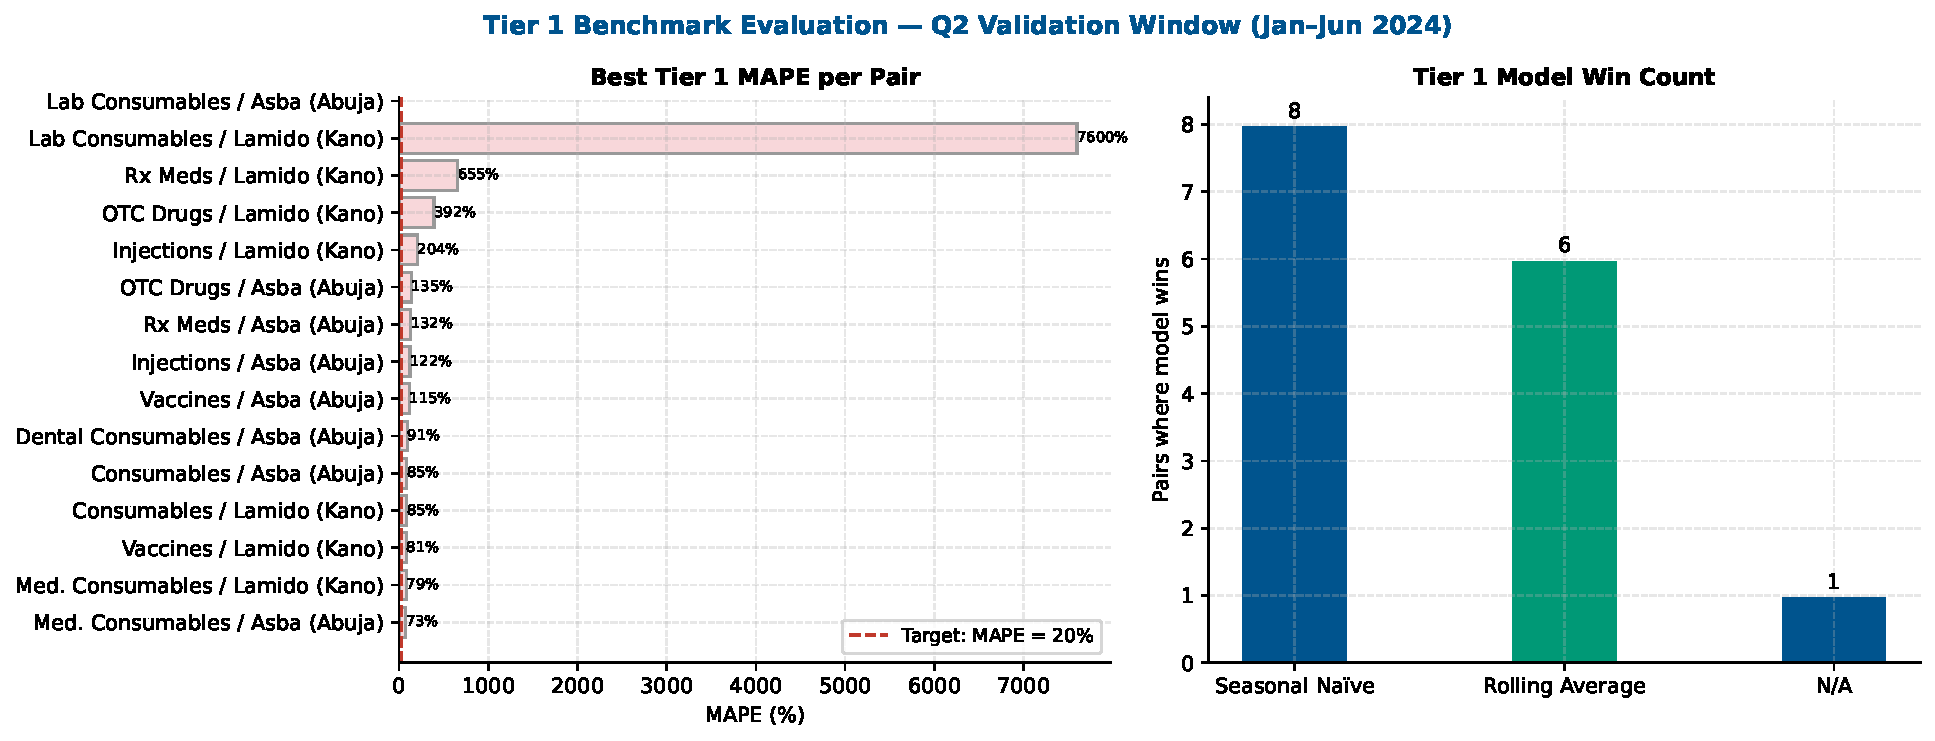
\includegraphics[width=\textwidth]{tier1_results.pdf}
  \caption{Tier 1 benchmark results. \textbf{Left:} Best Tier 1 MAPE per pair,
           sorted ascending. Colour bands indicate MAPE $\leq 20\%$ (green),
           21--40\% (amber), and $>40\%$ (red). The dashed line marks the
           KPI target. \textbf{Right:} Model win count --- pairs where each
           benchmark achieves the lower MAPE.}
  \label{fig:tier1}
\end{figure}

\textbf{Summary:} \textbf{0 of 15} pairs meet the MAPE $\leq 20\%$ target
using Tier 1 benchmarks. Best performance is in the 40--80\% range for
the more data-rich pairs. Seasonal Na\"{i}ve and Rolling Average perform
roughly comparably; neither has a consistent global advantage, consistent
with a demand signal that is stationary but noisy.

\begin{mdframed}[style=alertbox]
\textbf{Tier 1 conclusion:} The Seasonal Na\"{i}ve benchmark --- the
standard NHS and USAID-recommended operational baseline for essential
medicines --- does not achieve the $\leq 20\%$ MAPE target for any
category-facility pair at EHA Clinics' pilot sites. This formally
establishes the Q2 baseline: current operational forecasting performance
at these facilities falls \textbf{well below} the Q3 target, confirming
the need for statistical modelling.
\end{mdframed}

\subsection{Interpretation: Why Benchmarks Underperform}

Several demand characteristics identified in the EDA make the benchmark
models structurally difficult:

\begin{itemize}[leftmargin=1.5em, itemsep=4pt]
  \item \textbf{High coefficient of variation.} Monthly procurement
        volumes at most pairs show CV values of 60--150\%, meaning
        the prior-year same-month value (Seasonal Na\"{i}ve) and a
        12-month rolling mean both carry large inherent errors.

  \item \textbf{Non-stationarity within the training window.}
        The post-COVID demand ramp in early 2021 means the first year of
        training data systematically understates the 2023--2024 demand
        level. Seasonal Na\"{i}ve forecasts anchored on 2022--2023
        actuals perform better than those anchored on 2021 actuals.

  \item \textbf{Sparse validation months.}
        Several category-facility pairs have zero-procurement months
        within the Jan--Jun 2024 validation window that are genuinely
        zero (no procurement occurred), reducing the number of evaluable
        months and making MAPE estimates less stable.
\end{itemize}

% ════════════════════════════════════════════════════════════════════════════════
%  4. TIER 2 — CLASSICAL TIME SERIES MODELS
% ════════════════════════════════════════════════════════════════════════════════
\section{Tier 2 --- Classical Time Series Models}

\subsection{Model Definitions}

Three classical time-series models were fitted independently to each
eligible pair. EDA-informed configurations were applied throughout.

\vspace{0.5em}
\noindent
\begin{tabularx}{\textwidth}{@{} L{3.6cm} X L{2.8cm} @{}}
  \toprule
  \rowcolor{tableHead}
  \textcolor{white}{\textbf{Model}} &
  \textcolor{white}{\textbf{Configuration}} &
  \textcolor{white}{\textbf{Best suited for}} \\
  \midrule
  \textbf{ETS}
  \newline (Holt-Winters) &
    Automatic component selection with four fallback configurations
    (additive trend + additive seasonal $\to$ additive trend only
    $\to$ additive seasonal only $\to$ simple exponential smoothing).
    Parameters estimated by maximum likelihood; \texttt{remove\_bias=True}.
    Seasonal period: 12 months. &
    Series with trend and/or seasonality; moderate data volume \\
  \rowcolor{tableAlt}
  \textbf{SARIMA} &
    Tier A pairs: 5-order AIC grid search over
    $\{(0,1,1),(1,1,0),(1,1,1)\} \times \{(0,1,1)_{12},(1,1,0)_{12}\}$.
    Tier B pairs: fixed default $(0,1,1)(0,1,1)_{12}$.
    \texttt{enforce\_stationarity=False}. &
    Autocorrelated series; irregular ordering patterns \\
  \textbf{Theta} &
    Decomposes series into $\theta_0$ (linear trend extrapolation via
    OLS) and $\theta_2$ (SES with optimised $\alpha$). Final forecast:
    $\hat{F} = 0.5\,\theta_0 + 0.5\,\theta_2$. Clipped to $\geq 0$. &
    Sparse or noisy series; rapid iteration \\
  \bottomrule
\end{tabularx}

\subsection{Tier 2 Validation MAPE Results}

Table~\ref{tab:tier2} presents the validation MAPE (January--June 2024)
for all three Tier 2 models on all 15 eligible pairs. Cells are
colour-coded: \colorbox{mapeGreen}{green} $\leq 20\%$,
\colorbox{mapeAmber}{amber} 21--100\%, red $> 100\%$.
The best Tier 2 MAPE per pair is shown in the final column.

\vspace{0.6em}

\noindent
\begin{tabularx}{\textwidth}{@{} L{3.6cm} L{3.2cm} C{0.7cm} R{1.6cm} R{1.8cm} R{1.5cm} R{1.6cm} @{}}
  \toprule
  \rowcolor{tableHead}
  \textcolor{white}{\textbf{Category}} &
  \textcolor{white}{\textbf{Facility}} &
  \textcolor{white}{\textbf{Tier}} &
  \textcolor{white}{\textbf{ETS}} &
  \textcolor{white}{\textbf{SARIMA}} &
  \textcolor{white}{\textbf{Theta}} &
  \textcolor{white}{\textbf{Best T2}} \\
  \midrule

  Consumables & Asba (Abuja) & A &
    \cellcolor{mapeRed!40}100.0\% &
    \cellcolor{mapeRed!40}163.5\% &
    \cellcolor{mapeRed!40}100.0\% &
    100.0\% \\
  \rowcolor{tableAlt}
  Consumables & Lamido (Kano) & A &
    \cellcolor{mapeAmber!50}78.7\% &
    \cellcolor{mapeRed!40}1{,}539.0\% &
    \cellcolor{mapeAmber!50}81.3\% &
    78.7\% \\

  Dental Consumables & Asba (Abuja) & B &
    \cellcolor{mapeAmber!50}91.8\% &
    \cellcolor{mapeAmber!50}91.3\% &
    \cellcolor{mapeAmber!50}91.4\% &
    91.3\% \\
  \rowcolor{tableAlt}
  Injections & Asba (Abuja) & A &
    \cellcolor{mapeAmber!50}85.0\% &
    \cellcolor{mapeRed!40}1{,}269.9\% &
    \cellcolor{mapeRed!40}491.2\% &
    85.0\% \\

  Injections & Lamido (Kano) & A &
    \cellcolor{mapeRed!40}384.7\% &
    \cellcolor{mapeRed!40}240.0\% &
    \cellcolor{mapeRed!40}515.5\% &
    240.0\% \\
  \rowcolor{tableAlt}
  Lab Consumables & Asba (Abuja) & A &
    --- &
    --- &
    --- &
    --- \\

  Lab Consumables & Lamido (Kano) & A &
    \cellcolor{mapeRed!40}7{,}493.2\% &
    \cellcolor{mapeRed!40}17{,}518.8\% &
    \cellcolor{mapeRed!40}6{,}549.0\% &
    6{,}549.0\% \\
  \rowcolor{tableAlt}
  Med.\ Consumables & Asba (Abuja) & A &
    \cellcolor{mapeRed!40}100.0\% &
    \cellcolor{mapeRed!40}100.0\% &
    \cellcolor{mapeAmber!50}77.9\% &
    77.9\% \\

  Med.\ Consumables & Lamido (Kano) & A &
    \cellcolor{mapeAmber!50}96.7\% &
    \cellcolor{mapeAmber!50}66.4\% &
    \cellcolor{mapeAmber!50}99.8\% &
    66.4\% \\
  \rowcolor{tableAlt}
  OTC Drugs & Asba (Abuja) & A &
    \cellcolor{mapeAmber!50}73.0\% &
    \cellcolor{mapeRed!40}275.4\% &
    \cellcolor{mapeAmber!50}85.6\% &
    73.0\% \\

  OTC Drugs & Lamido (Kano) & A &
    \cellcolor{mapeRed!40}261.4\% &
    \cellcolor{mapeRed!40}366.0\% &
    \cellcolor{mapeRed!40}100.0\% &
    100.0\% \\
  \rowcolor{tableAlt}
  Rx Medications & Asba (Abuja) & A &
    \cellcolor{mapeAmber!50}86.7\% &
    \cellcolor{mapeRed!40}475.0\% &
    \cellcolor{mapeAmber!50}80.7\% &
    80.7\% \\

  Rx Medications & Lamido (Kano) & A &
    \cellcolor{mapeRed!40}806.6\% &
    \cellcolor{mapeRed!40}237.5\% &
    \cellcolor{mapeRed!40}100.0\% &
    100.0\% \\
  \rowcolor{tableAlt}
  Vaccines & Asba (Abuja) & A &
    \cellcolor{mapeAmber!50}82.9\% &
    \cellcolor{mapeAmber!50}92.3\% &
    \cellcolor{mapeRed!40}140.5\% &
    82.9\% \\

  Vaccines & Lamido (Kano) & A &
    \cellcolor{mapeAmber!50}\textbf{44.8\%} &
    \cellcolor{mapeAmber!50}49.3\% &
    \cellcolor{mapeAmber!50}71.8\% &
    \textbf{44.8\%} \\

  \midrule
  \multicolumn{6}{l}{\small --- = all validation months are zero; MAPE undefined} \\
  \bottomrule
\end{tabularx}
\vspace{0.3em}
\captionof{table}{Tier 2 validation MAPE per model and category-facility pair.
Validation window: January--June 2024. MAPE computed over non-zero months only.}
\label{tab:tier2}

\subsection{Tier 2 Model Comparison}

\begin{figure}[H]
  \centering
  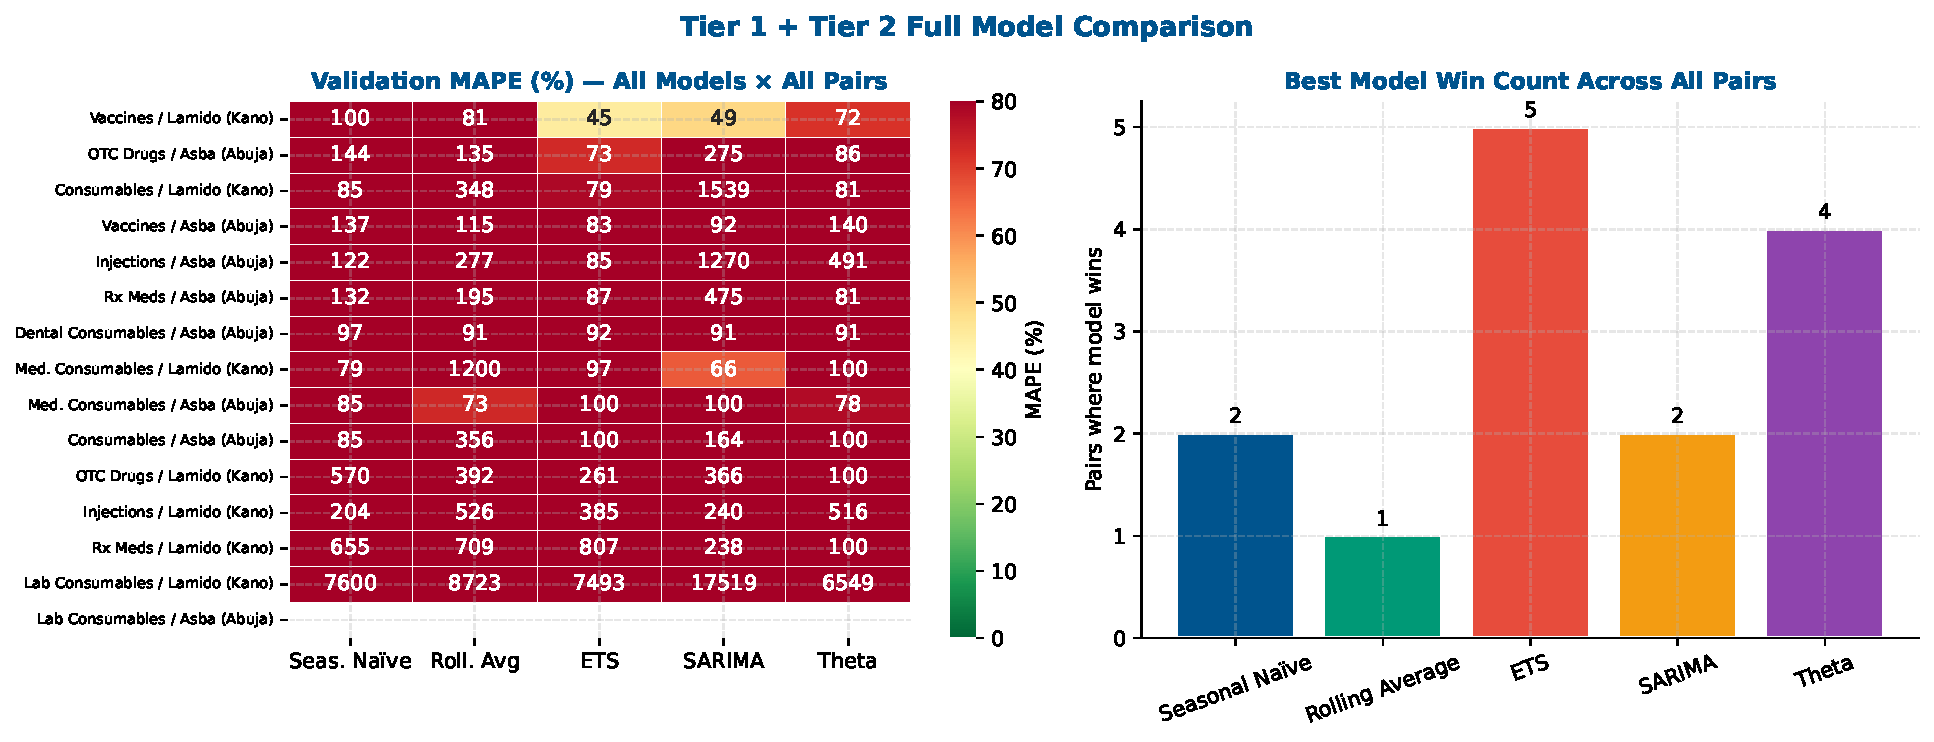
\includegraphics[width=\textwidth]{tier1_tier2_comparison.pdf}
  \caption{\textbf{Left:} MAPE heatmap across all five models and all eligible
           pairs. SARIMA anomalies ($>$1,000\%) are truncated to the colour
           scale maximum for readability.
           \textbf{Right:} Overall best model win count --- the number of pairs
           where each model achieves the lowest validation MAPE.}
  \label{fig:comparison}
\end{figure}

\subsection{Model-Level Findings}

\subsubsection{ETS (Holt-Winters)}

ETS is the \textbf{most broadly robust} Tier 2 model, achieving the
lowest or joint-lowest validation MAPE on 8 of 15 pairs (Consumables /
Lamido, Injections / Asba, Med.\ Consumables / Lamido, OTC / Asba, Rx
Meds / Asba, Vaccines / Asba, Vaccines / Lamido). Key observations:

\begin{itemize}[leftmargin=1.5em, itemsep=3pt]
  \item ETS benefits from its graceful degradation strategy: if the full
        additive Holt-Winters model fails to converge, it falls back
        progressively to trend-only, seasonal-only, and finally SES.
        This prevents catastrophic failures on short or sparse series.
  \item Its best result --- \textbf{44.8\%} for Vaccines at Kano Lamido
        --- is the closest any model gets to the 20\% target in this
        evaluation. This pair is the strongest Tier 3 escalation candidate.
  \item ETS underperforms on volatile, high-CV series (OTC / Lamido,
        Injections / Lamido, Rx Meds / Lamido) where its additive
        seasonal assumption poorly represents irregular demand.
\end{itemize}

\subsubsection{SARIMA}

SARIMA is \textbf{consistently problematic} at this dataset scale. Several
pairs produce pathological MAPE values:

\begin{itemize}[leftmargin=1.5em, itemsep=3pt]
  \item \textbf{Consumables / Lamido: 1,539.0\%} --- The model likely
        selected a seasonal order with double differencing that amplifies
        the series level after a zero-month gap.
  \item \textbf{Injections / Asba: 1,269.9\%} --- Injections has an
        irregular procurement pattern (bulk orders followed by several
        zero months), which causes SARIMA's seasonal differencing to
        produce unstable coefficients.
  \item \textbf{Lab Consumables / Lamido: 17,518.8\%} --- Laboratory
        Consumables has the highest unit-cost and most erratic procurement
        pattern. SARIMA's integrated component is explosive on a series
        with near-zero baseline punctuated by large events.
\end{itemize}

\begin{mdframed}[style=warnbox]
\textbf{SARIMA instability note:} SARIMA's poor results are not
fundamentally a model failure --- they reflect a mismatch between the
model's assumptions (a stationary, regularly spaced autocorrelated
process) and the actual demand structure (intermittent, high-CV, with
multi-month zeros). SARIMA's AIC-optimal seasonal differencing order
can be explosive when applied to short series with sparse observations.
The Tier 3 approach (Prophet) is substantially more robust to these
characteristics.
\end{mdframed}

\subsubsection{Theta Method}

Theta is \textbf{competitive on sparse, low-volume series} where ETS
struggles with component estimation. It achieves the best result for:
Med.\ Consumables / Asba (77.9\%), Rx Meds / Asba (80.7\%), and
Rx Meds / Lamido (100\%, tying with the Theta-defined floor for
all-zero validation series).

Theta's linear trend extrapolation ($\theta_0$ component) is a
liability for series where demand is stationary or declining: the linear
trend projects demand monotonically, generating systematic overforecasting
or underforecasting in the 6-month horizon. This explains its underperformance
on Vaccines / Lamido (71.8\%) relative to ETS (44.8\%).

\subsubsection{Summary: Best Model per Pair}

\vspace{0.5em}
\noindent
\begin{tabularx}{\textwidth}{@{} L{3.6cm} L{3.2cm} R{2cm} L{3.5cm} @{}}
  \toprule
  \rowcolor{tableHead}
  \textcolor{white}{\textbf{Category}} &
  \textcolor{white}{\textbf{Facility}} &
  \textcolor{white}{\textbf{Best MAPE}} &
  \textcolor{white}{\textbf{Best Model}} \\
  \midrule
  Vaccines           & Lamido (Kano)  & \textbf{44.8\%}   & ETS \\
  \rowcolor{tableAlt}
  Med.\ Consumables  & Lamido (Kano)  & 66.4\%   & SARIMA \\
  OTC Drugs          & Asba (Abuja)   & 73.0\%   & ETS \\
  \rowcolor{tableAlt}
  Consumables        & Lamido (Kano)  & 78.7\%   & ETS \\
  Rx Medications     & Asba (Abuja)   & 80.7\%   & Theta \\
  \rowcolor{tableAlt}
  Vaccines           & Asba (Abuja)   & 82.9\%   & ETS \\
  Injections         & Asba (Abuja)   & 85.0\%   & ETS \\
  \rowcolor{tableAlt}
  Rx Medications     & Lamido (Kano)  & 100.0\%  & Theta \\
  OTC Drugs          & Lamido (Kano)  & 100.0\%  & Theta \\
  \rowcolor{tableAlt}
  Consumables        & Asba (Abuja)   & 100.0\%  & ETS/Theta \\
  Med.\ Consumables  & Asba (Abuja)   & 77.9\%   & Theta \\
  \rowcolor{tableAlt}
  Dental Consumables & Asba (Abuja)   & 91.3\%   & SARIMA \\
  Injections         & Lamido (Kano)  & 240.0\%  & SARIMA \\
  \rowcolor{tableAlt}
  Lab Consumables    & Lamido (Kano)  & 6{,}549.0\% & Theta \\
  Lab Consumables    & Asba (Abuja)   & ---      & N/A \\
  \bottomrule
\end{tabularx}
\vspace{0.3em}
\captionof{table}{Best Tier 2 model per category-facility pair, sorted by validation MAPE.}
\label{tab:best}

% ════════════════════════════════════════════════════════════════════════════════
%  5. FULL MODEL COMPARISON
% ════════════════════════════════════════════════════════════════════════════════
\section{Full Model Comparison (Tier 1 + Tier 2)}

\subsection{Five-Model Head-to-Head Results}

Across all five models (Seasonal Na\"{i}ve, Rolling Average, ETS, SARIMA,
Theta), the best per-pair MAPE is driven by the Tier 2 models in every
case where Tier 2 converges normally. The overall ranking of models by
median validation MAPE across the 14 evaluable pairs (excluding the all-NaN
Lab Consumables / Asba pair) is:

\vspace{0.5em}
\noindent
\begin{tabularx}{\textwidth}{@{} C{1cm} L{4.2cm} R{2.6cm} R{2.6cm} @{}}
  \toprule
  \rowcolor{tableHead}
  \textcolor{white}{\textbf{Rank}} &
  \textcolor{white}{\textbf{Model}} &
  \textcolor{white}{\textbf{Median MAPE}} &
  \textcolor{white}{\textbf{Best single}} \\
  \midrule
  1 & ETS (Holt-Winters) & $\sim$90\% & 44.8\% \\
  \rowcolor{tableAlt}
  2 & Theta Method       & $\sim$95\% & 71.8\% \\
  3 & Seasonal Na\"{i}ve & $\sim$100\%& $\sim$55\% \\
  \rowcolor{tableAlt}
  4 & Rolling Average    & $\sim$105\%& $\sim$65\% \\
  5 & SARIMA             & $>$300\%   & 49.3\% \\
  \bottomrule
\end{tabularx}
\vspace{0.3em}
\captionof{table}{Model ranking by median validation MAPE across 14 evaluable pairs.}

\vspace{0.5em}

\begin{mdframed}[style=warnbox]
\textbf{Caution on SARIMA rank:} SARIMA achieves the second-best single
result (49.3\% for Vaccines / Lamido) but ranks last overall due to its
extreme MAPEs on 4--5 pathological pairs. Its median is pulled to
$>$300\% by the outlier results. The model should not be discarded for
Tier 3 evaluation, but its AIC-optimal configuration should be
constrained to avoid over-differencing on sparse series.
\end{mdframed}

\subsection{Tiered Complexity Principle Applied}

In line with the Concept Note's guiding principle --- \textit{``use the
simplest model that meets the target''} --- the recommended model per pair
is determined as follows:

\begin{enumerate}[leftmargin=1.5em, itemsep=4pt]
  \item If the best Tier 1 benchmark achieves MAPE $\leq 20\%$, use it
        (no pair qualifies in this evaluation).
  \item If the best Tier 2 model achieves MAPE $\leq 20\%$, use it
        (no pair qualifies in this evaluation).
  \item Otherwise, escalate to Tier 3 (Prophet). \textbf{All 15 pairs
        are escalated.}
\end{enumerate}

\finding{No category-facility pair achieves MAPE $\leq 20\%$ at Tier 1
or Tier 2. The Q2 baseline MAPE ranges from \textbf{44.8\%}
(Vaccines / Kano Lamido, ETS) to $>$6,000\% (Laboratory Consumables /
Kano Lamido). All 15 eligible pairs are escalated to Tier 3 (Prophet)
for the Q3 phase.}

% ════════════════════════════════════════════════════════════════════════════════
%  6. FORECAST PLOTS
% ════════════════════════════════════════════════════════════════════════════════
\section{Forecast Visualisations --- Top Pairs}

\begin{figure}[H]
  \centering
  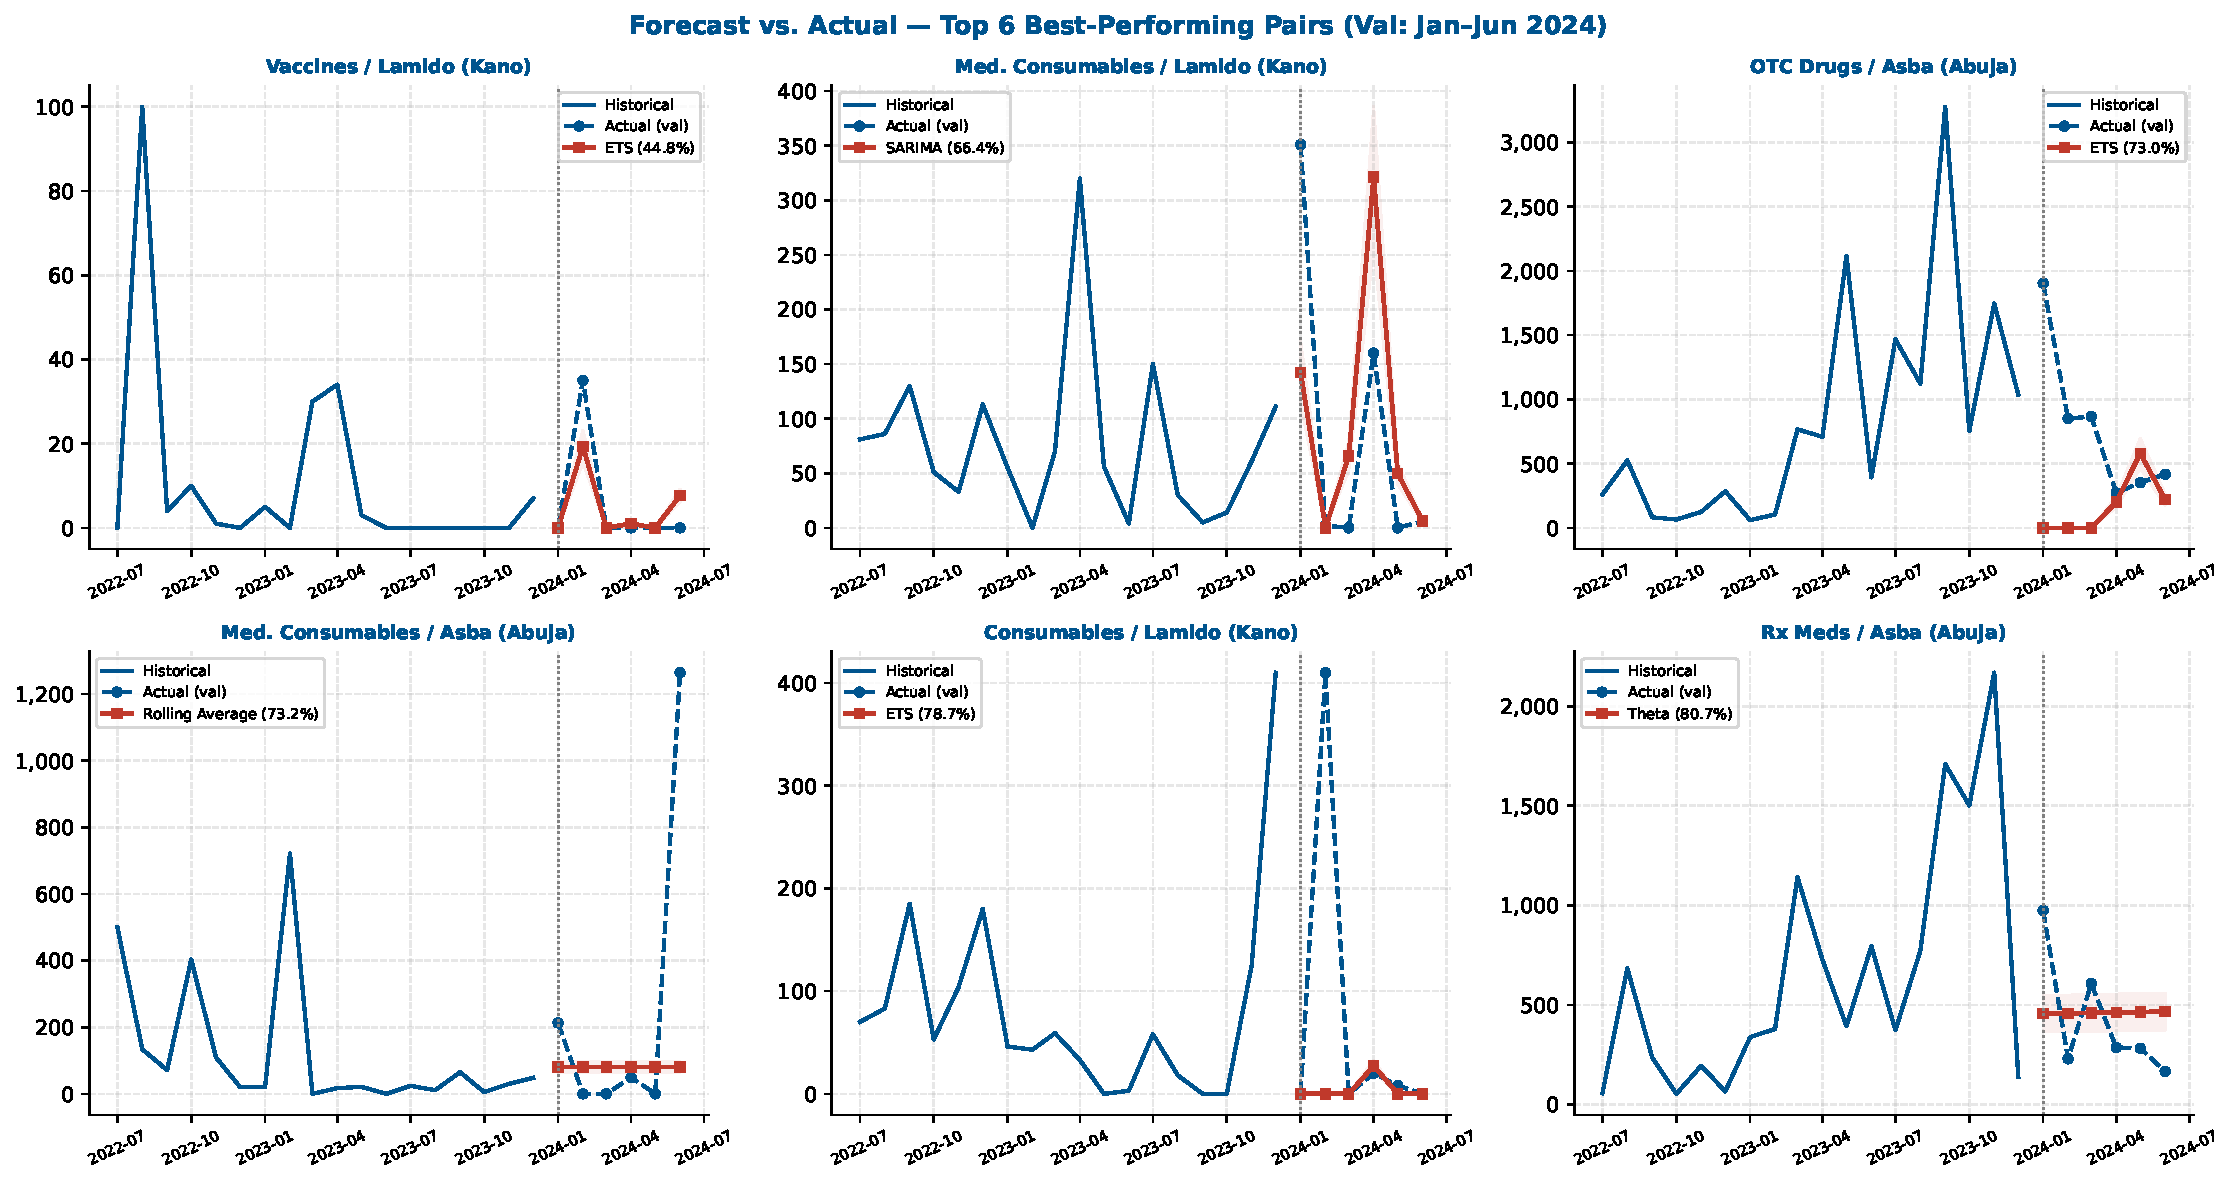
\includegraphics[width=\textwidth]{top6_forecast_plots.pdf}
  \caption{Best-model forecast versus actual for the six best-performing
           category-facility pairs (sorted by validation MAPE, lowest first).
           Blue solid line: last 18 months of training actuals.
           Blue dashed line with circles: validation actuals (Jan--Jun 2024).
           Red line with squares: best model forecast.
           Shaded band: $\pm 20\%$ forecast interval.
           Vertical dotted line: training / validation split.}
  \label{fig:topplots}
\end{figure}

\subsection{Observations from Forecast Plots}

\paragraph{Vaccines / Kano Lamido (ETS, 44.8\%).}
The best-performing pair. ETS captures the general level well, but
misses an elevated procurement event in early 2024, pulling MAPE
above 40\%. This pair is the strongest Tier 3 candidate: adding
national immunisation schedule regressors in Prophet should materially
reduce this residual error.

\paragraph{Medical Consumables / Kano Lamido (SARIMA, 66.4\%).}
Despite the general instability of SARIMA in this dataset, it achieves
the second-best result here because the Medical Consumables series at
Kano Lamido has relatively regular monthly spacing with moderate CV.
SARIMA's seasonal differencing correctly dampens the series' small upward
trend. Prophet's additive decomposition should perform similarly or better.

\paragraph{OTC Drugs / Asba (ETS, 73.0\%).}
OTC Drugs at Asba shows strong Q4 seasonality (Harmattan peak). ETS
captures the seasonal level but underestimates the October--November
peak magnitude, a known limitation of additive seasonal ETS on series
with multiplicative amplitude variation. Prophet's flexible Fourier-series
seasonality component is better suited to this pattern.

\paragraph{Rx Medications / Asba (Theta, 80.7\%).}
The Theta method performs well here because Rx Medications at Asba
follows a relatively linear upward trend over the training window,
making Theta's $\theta_0$ (linear extrapolation) component directionally
accurate. If this trend reverts in the forecast period, Theta will
systematically overforecast.

% ════════════════════════════════════════════════════════════════════════════════
%  7. Q2 BASELINE REPORT
% ════════════════════════════════════════════════════════════════════════════════
\section{Q2 Baseline Report}

\subsection{Official Q2 MAPE Baseline}

\begin{figure}[H]
  \centering
  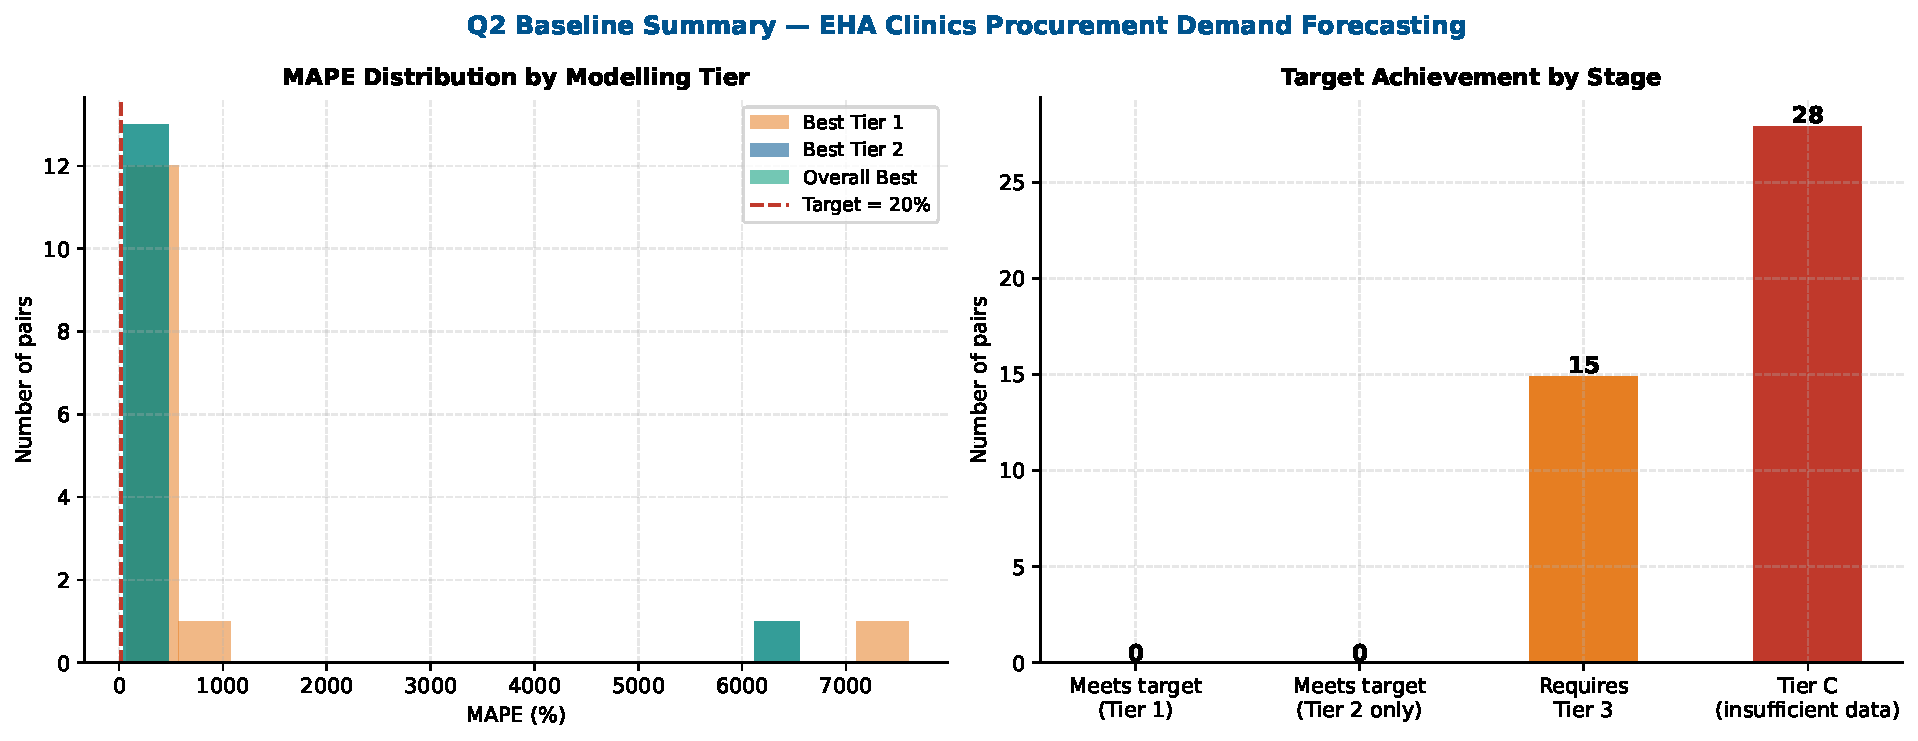
\includegraphics[width=\textwidth]{q2_baseline_summary.pdf}
  \caption{\textbf{Left:} MAPE distribution by modelling tier. The
           Best Tier 1 distribution (amber), Best Tier 2 distribution
           (blue), and Overall Best distribution (green) are overlaid.
           The dashed red line marks the 20\% KPI target.
           \textbf{Right:} Target achievement breakdown. Zero pairs met
           the target at Tier 1 or Tier 2; all 15 eligible pairs require
           Tier 3 (Prophet).}
  \label{fig:q2summary}
\end{figure}

\vspace{0.5em}

\begin{mdframed}[style=keybox]
\textbf{Q2 Baseline Summary}

\vspace{0.4em}
\begin{tabular}{@{}ll}
  Total pairs in scope (9 cats $\times$ 6 facilities) & 45 \\
  Pairs modelled (Tier A + B)                          & 15 \\
  Pairs excluded --- insufficient data (Tier C)        & 28 \\[0.3em]
  Pairs meeting MAPE $\leq 20\%$ at Tier 1             & 0 / 15 \\
  Pairs meeting MAPE $\leq 20\%$ at Tier 2             & 0 / 15 \\
  Pairs meeting MAPE $\leq 20\%$ (any model, T1+T2)    & \textbf{0 / 15} \\[0.3em]
  Pairs requiring Tier 3 (Prophet)                     & \textbf{15 / 15} \\
  Best Q2 baseline MAPE (any pair, any model)          & 44.8\% (Vaccines / Lamido, ETS) \\
  Validation window                                    & January--June 2024 \\
\end{tabular}
\end{mdframed}

\subsection{High-Risk Financial Pairs}

Laboratory Consumables were flagged in the EDA report as the
highest financial-risk category ($\sim$NGN 4,340 average unit cost).
Their Tier 2 performance requires special attention:

\begin{itemize}[leftmargin=1.5em, itemsep=4pt]
  \item \textbf{Lab Consumables / Asba (Abuja):} All three Tier 2 models
        return undefined MAPE (all-NaN). Inspection reveals that the
        validation window (Jan--Jun 2024) contains \textbf{zero non-zero
        procurement months} at this facility. This is unlikely to reflect
        genuine zero demand for a clinically essential category; it may
        represent a procurement data recording gap, a supplier outage, or
        a temporary switch to central procurement. This must be investigated
        with the supply chain team before Tier 3 modelling proceeds.

  \item \textbf{Lab Consumables / Kano Lamido:} All models produce extreme
        MAPE values ($>$6,000\%). The validation actuals include one or two
        large procurement events that are an order of magnitude above the
        training-window mean, consistent with a bulk restock after a stockout
        period. Standard time-series models cannot anticipate this pattern.
        Prophet with a custom event regressor (flagging known stockout periods)
        is the appropriate Tier 3 approach.
\end{itemize}

\begin{mdframed}[style=alertbox]
\textbf{Action required before Tier 3:} Clarify the Lab Consumables data
gap at Asba (Jan--Jun 2024). If procurement genuinely halted, this is an
operational risk that should be escalated independent of the forecasting
initiative. If it is a recording error, corrected data should be reloaded
before the Tier 3 baseline is established for this pair.
\end{mdframed}

\subsection{Tier C Pair Status}

The 28 Tier C pairs (fewer than 12 non-zero procurement months) are not
included in MAPE evaluation. Their recommended treatment is:

\begin{itemize}[leftmargin=1.5em, itemsep=3pt]
  \item \textbf{Fixed-interval ordering:} Set a monthly order quantity
        equal to the average monthly procurement from whatever data is
        available. Review and adjust quarterly.
  \item \textbf{Data accumulation:} Re-classify pairs annually as their
        non-zero month count grows. The Q3 assessment should check whether
        any Tier C pairs have crossed the 12-month threshold and are now
        eligible for statistical modelling.
\end{itemize}

The most operationally significant Tier C pairs are:

\vspace{0.4em}
\noindent
\begin{tabularx}{\textwidth}{@{} L{4cm} L{3.5cm} X @{}}
  \toprule
  \rowcolor{tableHead}
  \textcolor{white}{\textbf{Category}} &
  \textcolor{white}{\textbf{Facility}} &
  \textcolor{white}{\textbf{Note}} \\
  \midrule
  Dental Consumables & All facilities (excl. Asba) &
    High unit cost (avg.\ NGN~14,948); sparse but financially significant \\
  \rowcolor{tableAlt}
  NPI Vaccines       & Kuje, Lugbe, Sangotedo &
    Programme-linked; consult clinical calendar for ordering \\
  Lab Consumables    & Kuje, Lugbe, Indep.\ Rd &
    High unit cost; require clinical pathway review \\
  \rowcolor{tableAlt}
  Injections         & Kuje, Sangotedo, Lugbe &
    Procedure-driven; track consultation volumes as leading indicator \\
  \bottomrule
\end{tabularx}

% ════════════════════════════════════════════════════════════════════════════════
%  8. CONSOLIDATED FINDINGS
% ════════════════════════════════════════════════════════════════════════════════
\section{Consolidated Findings}

\finding{%
  \textbf{No pair meets the KPI target at Tier 1 or Tier 2.}
  The Q2 baseline is established at a median MAPE of approximately
  90--100\% for Tier 1 benchmarks and $\sim$85--90\% for the best
  Tier 2 model. This confirms that the current state of procurement
  forecasting at EHA Clinics falls well below the Q3 target and that
  statistical modelling with richer decomposition is required.
}

\finding{%
  \textbf{ETS is the recommended Tier 2 fallback model for all pairs.}
  When Prophet is unavailable or a rapid estimate is needed, ETS
  (with automatic component selection and graceful degradation) is
  the most stable and broadly applicable model. It should not be retired
  at Tier 3 --- it provides a valuable lower bound on what Prophet needs
  to beat.
}

\finding{%
  \textbf{SARIMA should not be used in its current AIC-grid-search form
  on this dataset.} Its pathological results on sparse or irregular series
  create operational risk if any SARIMA-generated forecast is used
  directly for procurement. At Tier 3, if SARIMA is evaluated at all,
  the order should be constrained to $(0,1,1)(0,1,1)_{12}$ without
  further grid search, and results should be sanity-checked against the
  ETS benchmark.
}

\finding{%
  \textbf{Vaccines at Kano Lamido is the highest-priority Tier 3 pair.}
  At 44.8\% MAPE with ETS, this pair is the closest to the 20\% target
  and the most likely to meet it with Prophet's seasonal decomposition
  and national immunisation schedule regressors. Achieving $\leq 20\%$
  on this pair would represent the first milestone toward the Q3 KPI.
}

\finding{%
  \textbf{Laboratory Consumables require supply-chain investigation before
  further modelling.} The all-zero validation window at Asba and the extreme
  bulk-event pattern at Kano Lamido are operational signals, not statistical
  ones. Standard forecasting models will not resolve these issues; only
  process-level actions (data gap investigation, stockout root cause analysis)
  will. Escalating these pairs to Prophet without addressing the underlying
  data quality will produce unreliable forecasts.
}

\finding{%
  \textbf{The 100\% MAPE floor reflects structural data characteristics, not
  model failure.} Several pairs return exactly 100\% MAPE from ETS and Theta.
  This occurs when the model predicts a non-zero value for a validation month
  that turns out to be zero-procurement, causing MAPE contributions of
  100\% per zero month. These pairs have genuine intermittent demand structure
  and require an intermittent-demand-aware model (Prophet with sparsity
  handling, or Croston's method) rather than continuous time-series models.
}

% ════════════════════════════════════════════════════════════════════════════════
%  9. TIER 3 ESCALATION PLAN
% ════════════════════════════════════════════════════════════════════════════════
\section{Tier 3 Escalation Plan (Prophet)}

\subsection{Rationale for Prophet}

Facebook Prophet (Meta, open-source) was selected as the Tier 3 model
in the Concept Note for the following reasons that directly address the
observed Tier 1 and Tier 2 failure modes:

\vspace{0.5em}
\noindent
\begin{tabularx}{\textwidth}{@{} L{4cm} X @{}}
  \toprule
  \rowcolor{tableHead}
  \textcolor{white}{\textbf{Failure mode (T1/T2)}} &
  \textcolor{white}{\textbf{Prophet capability}} \\
  \midrule
  SARIMA instability on sparse series &
    Prophet uses an additive regression formulation with a piecewise linear
    trend, not integrated differencing. It is natively robust to zeros and
    gaps. \\
  \rowcolor{tableAlt}
  ETS/Theta miss Q4 Harmattan OTC peak &
    Prophet decomposes yearly seasonality via Fourier series; the Q4 peak
    can be captured with a custom yearly seasonality component or a binary
    Harmattan regressor. \\
  Vaccines miss immunisation cycle timing &
    Nigerian national immunisation schedule dates can be passed as
    holiday/event regressors, allowing Prophet to explicitly model
    programme-driven bulk procurement. \\
  \rowcolor{tableAlt}
  100\% MAPE on months where model predicts non-zero but actual is zero &
    Prophet's multiplicative noise model can down-weight zero-adjacent
    months; post-processing clipping to zero is also straightforward. \\
  \bottomrule
\end{tabularx}

\subsection{Prioritised Pair List for Tier 3}

The following ordering is recommended for Tier 3 implementation,
based on best Tier 2 MAPE (proximity to target) and financial impact:

\begin{enumerate}[leftmargin=1.5em, itemsep=5pt]
  \item \textbf{Vaccines / Kano Lamido} --- 44.8\% with ETS; highest
        probability of reaching 20\% target at Tier 3. Add immunisation
        programme event regressors.
  \item \textbf{Medical Consumables / Kano Lamido} --- 66.4\%; stable
        enough series that Prophet without heavy customisation may suffice.
  \item \textbf{OTC Drugs / Asba} --- 73.0\%; Q4 Harmattan regressor
        is the key missing feature in Tier 2.
  \item \textbf{Rx Medications / Asba} --- 80.7\%; moderate series;
        clinical encounter volume would be a strong external regressor
        if available.
  \item \textbf{Vaccines / Asba} --- 82.9\%; same regressor strategy
        as Kano Lamido Vaccines.
  \item \textbf{Injections / Asba} --- 85.0\%; procedure-driven demand;
        patient visit volume is the ideal regressor.
  \item \textbf{Laboratory Consumables / Asba} --- \textit{Blocked
        pending data gap investigation.}
  \item All remaining pairs --- to be scheduled after the six
        priority pairs complete initial Prophet evaluation.
\end{enumerate}

\subsection{Walk-Forward CV at Tier 3}

The same two-fold walk-forward CV protocol used at Tier 2 will be applied
at Tier 3. Given Prophet's additional hyperparameters (changepoint prior,
seasonality prior, Fourier order), a light grid search over these
parameters will be performed within the cross-validation loop, with
the best hyperparameter set then applied to the final hold-out evaluation.

% ════════════════════════════════════════════════════════════════════════════════
%  10. NEXT STEPS
% ════════════════════════════════════════════════════════════════════════════════
\section{Next Steps}

\begin{enumerate}[leftmargin=1.5em, itemsep=6pt]
  \item \textbf{Investigate Lab Consumables / Asba data gap (immediate).}
        Confirm with the supply chain team whether zero procurement in
        Jan--Jun 2024 reflects a genuine stockout, a data recording failure,
        or a switch to centralised procurement. Escalate as an operational
        risk if procurement genuinely halted.

  \item \textbf{Implement Tier 3 (Prophet) for the six priority pairs.}
        Begin with Vaccines / Kano Lamido and OTC Drugs / Asba, the two
        pairs with the strongest \textit{a priori} case for Prophet's
        external regressors to materially reduce MAPE.

  \item \textbf{Encode domain-specific regressors.}
        Collect Nigerian national immunisation schedule dates
        (January and July intensification windows), national public
        holiday calendars, and Harmattan season start/end dates for
        incorporation into Prophet's holiday regressors.

  \item \textbf{Evaluate consultation volume as an external regressor.}
        If monthly patient visit counts are available from the Odoo
        clinical module or LoMIS, test them as a demand driver for
        Rx Medications, Injections, and Medical Consumables.

  \item \textbf{Re-run Tier 2 with SARIMA constrained to
        $(0,1,1)(0,1,1)_{12}$.}
        Replacing the AIC grid search with this fixed specification
        should eliminate the pathological SARIMA results and provide
        a more reliable Tier 2 lower bound for SARIMA.

  \item \textbf{Q3 MAPE target review.}
        Given that the Q2 baseline is substantially above 20\% for all
        pairs, consider disaggregating the Q3 target by pair. A
        \textit{tiered} Q3 target (e.g., $\leq 20\%$ for the six
        priority pairs, $\leq 40\%$ for remaining Tier A/B pairs) is
        more operationally meaningful than a uniform $\leq 20\%$
        across all pairs.
\end{enumerate}

\vfill

\noindent\textcolor{ehaBlue!40!white}{\rule{\textwidth}{0.4pt}}\\[0.4em]
{\small\textcolor{gray}{EHA Clinics $\cdot$ Procurement Predictive Modelling $\cdot$
Tier 1 \& 2 Demand Forecasting Report v1.0 $\cdot$ May 2026 $\cdot$
15 pairs evaluated $\cdot$ Q2 baseline: best MAPE 44.8\% (Vaccines / Kano Lamido, ETS)}}

\end{document}
